\documentclass{article}

\usepackage{amssymb,amsmath,amsthm,tikz,tcolorbox,extpfeil,makecell}

\usetikzlibrary{matrix,backgrounds,patterns,positioning}

\setlength{\parindent}{0pt}
\setlength{\parskip}{1em}

\newcommand{\bN}{\mathbb{N}}
\newcommand{\bP}{\mathbb{P}}
\newcommand{\bZ}{\mathbb{Z}}
\newcommand{\bQ}{\mathbb{Q}}
\newcommand{\bR}{\mathbb{R}}
\newcommand{\bC}{\mathbb{C}}
\newcommand{\cP}{\mathcal{P}}
\newcommand{\bijection}{\xrightarrow{\sim}}
\newcommand{\bijectivemap}[1]{\xmapsto[#1]{\sim}}

\newtheorem{theorem}{Theorem}[section]
\newtheorem{corollary}{Corollary}[theorem]
\newtheorem{lemma}[theorem]{Lemma}
\title{Posets}
\author{Hiten Tandon}
\date{}

\begin{document}
\maketitle

\section{Notation}

\begin{description}
  \item[$\bN$]= Natural Numbers
  \item[$\bP$]= Positive Integers
  \item[$\bZ$]= Integers
  \item[$\bR$]= Real Numbers
  \item[$\bC$]= Complex Numbers
  \item[R]= Commutative Unital RING
  \item[$\cP$]= Set of all Prime numbers
  \item[{$[a, b]$}]= $\{x \in \bZ \left| a \le x \le b\right.\}$
  \item[{$[a]$}]= $[1, a]$
  \item[{$\bijection$}]= Used to represent a bijective function
    (one-one mapping)
  \item[{$\bijectivemap\phi$}]= Used to show the bijective mapping
    under the function $\phi$
  \item[$\hat0$]= Smallest element of the Poset
  \item[$\hat1$]= Greatest element of the Poset
  \item[$\le_X$]= less than or equal, in the poset $X$.
  \item[$n(\dots)$]= cardinality of the expression in the parenths.
\end{description}

\section{Partially Ordered Sets / Posets}

A partially ordered set also known as a Poset is a pair of a set $P$
and a relation $\le \colon P^2$ s.t it staisfies:
\begin{enumerate}
  \item $\forall x \in P. x \le x$ (Reflexivity)
  \item $\forall x, y, z \in P, x \le y, y \le z. x \le z.$ (Transitivity)
  \item $\forall x, y \in P, x \le y, y \le x. x = y.$ (Anti-symmetry)
\end{enumerate}

Common examples of Posets include
\begin{enumerate}
  \item all subsets of $(\bC, \le)$
  \item $(\bP, \mid)$
  \item $\forall a, b \in \bZ. [a,b]$
  \item $\forall X: \text{Set}. (2^X, \subseteq)$
  \item $\left(\bR^2, \left\{(x, y), (x', y') \in \bR^2 \left| x \le
    x', y \le y'\right.\right\}\right)$
\end{enumerate}

\begin{tcolorbox}[colframe=blue!50, title=Chains and Anti-chains]
  A Poset $(P, \le)$ is called a chain if $\forall x, y \in P, x \le
  y \text{ or } y \le x$.
  Common examples of this would include $\bN, \bP, \bR$ and their subsets.
  \tcblower
  A Poset $(P, \le)$ is called an anti-chain if $\forall x, y \in P,
  x \le y \iff y \le x$.
  A common example of an antichain would be the set of all human
  laguages, or programming languages.
\end{tcolorbox}

\subsection{Hasse Diagrams}
A common way to graphically represent a Poset is by using Hasse diagrams.
A Hasse diagram is a graphical representation of a Poset where the
following conditions are met:
\begin{enumerate}
  \item Vertices of the graph represent an element of the poset $P$
  \item There is an edge from $x$ to $y$ if $x$ covers $y$.
\end{enumerate}

Cover here means the following:
If $\forall x, y \in P. \nexists z \in P, z \leq x, y \leq z, x \neq
z, y \neq z.$ then $x$ is said to cover $y$.

Generally, Hasse diagrams are drawn without arrows, by placing the
covering element physically above the covered element.

For example:
Consider the Poset $(2^{[2]}, \subseteq)$
The containment relation can be listed as:

\begin{center}
  \begin{tabular}{ |c|c| }
    \hline
    $X$ & $Y \in 2^{[2]} \text{ s.t. } X \subseteq Y$\\
    \hline
    $\emptyset$ & $\emptyset, \{1\}, \{2\}, \{1, 2\}$\\
    $\{1\}$ & $\{1\}, \{1, 2\}$\\
    $\{2\}$ & $\{2\}, \{1, 2\}$\\
    $\{1, 2\}$ & $\{1, 2\}$\\
    \hline
  \end{tabular}
\end{center}

This would be drawn in a Hasse diagram as follows:

\begin{tcolorbox}[colframe=orange!50, title = Hasse diagram of $2^X$]
  \begin{center}
    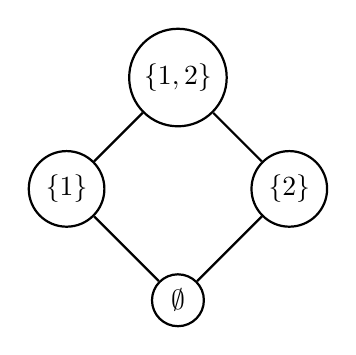
\begin{tikzpicture}[main/.style = {draw, circle}, node distance =
      20mm, thick]
      \node[main] (0) {$\emptyset$};
      \node[main] (1) [above left of=0] {$\{1\}$};
      \node[main] (2) [above right of=0] {$\{2\}$};
      \node[main] (3) [above right of = 1] {$\{1, 2\}$};

      \draw (0) -- (1);
      \draw (0) -- (2);
      \draw (1) -- (3);
      \draw (2) -- (3);
    \end{tikzpicture}
  \end{center}
  \tcblower
  Note that, there is no edge connecting $\emptyset$ with $\{1, 2\}$.
  This is because we draw an edge from
  covered vertices to covering verticies. However, for a vertex to
  cover another, we don't just say that
  it should exist as the RHS of the relation, it is imperative that
  there exists no middle man
  which could cover it instead. In the case of $\emptyset$ and $\{1,
  2\}$ there are two vertices which can
  cover $\emptyset$ which are $\{1\}$ and $\{2\}$.
\end{tcolorbox}

Similarly now lets look at Hasse diagram for $([3], \subseteq)$

We get the table as:
\begin{center}
  \begin{tabular}{ |c|c| }
    \hline
    $X$ & $Y \in 2^{[2]} \text{ s.t. } X \subseteq Y$\\
    \hline
    $\emptyset$ & $\emptyset, \{1\}, \{2\}, \{3\}, \{1, 2\}, \{1,
    3\}, \{2, 3\}, \{1, 2, 3\}$\\
    $\{1\}$ & $\{1\}, \{1, 2\}, \{1, 3\}, \{1, 2, 3\}$\\
    $\{2\}$ & $\{2\}, \{1, 2\}, \{2, 3\}, \{1, 2, 3\}$\\
    $\{3\}$ & $\{3\}, \{1, 3\}, \{2, 3\}, \{1, 2, 3\}$\\
    $\{1, 2\}$ & $\{1, 2\}, \{1, 2, 3\}$\\
    $\{1, 3\}$ & $\{1, 3\}, \{1, 2, 3\}$\\
    $\{2, 3\}$ & $\{2, 3\}, \{1, 2, 3\}$\\
    $\{1, 2, 3\}$ & $\{1, 2, 3\}$\\
    \hline
  \end{tabular}
\end{center}

\begin{tcolorbox}[colframe=orange!50, title = Hasse diagram of $2^X$]
  \begin{center}
    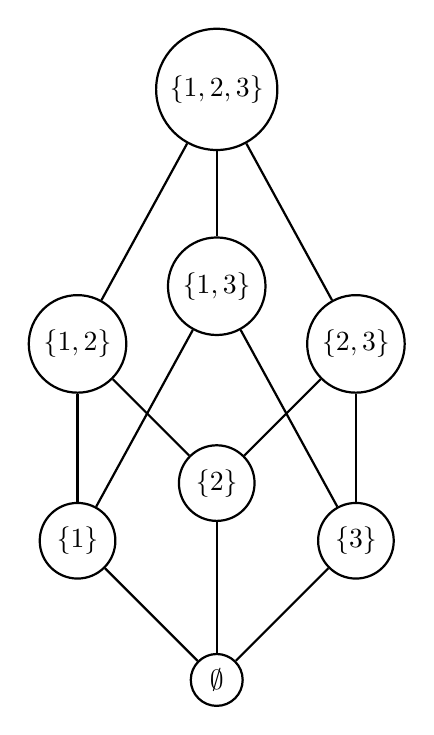
\begin{tikzpicture}[main/.style = {draw, circle}, node distance =
      25mm, thick]
      \node[main] (0) {$\emptyset$};
      \node[main] (1) [above left of=0] {$\{1\}$};
      \node[main] (2) [above of=0] {$\{2\}$};
      \node[main] (3) [above right of=0] {$\{3\}$};
      \node[main] (4) [above of=1] {$\{1, 2\}$};
      \node[main] (5) [above of=2] {$\{1, 3\}$};
      \node[main] (6) [above of=3] {$\{2, 3\}$};
      \node[main] (7) [above of=5] {$\{1, 2, 3\}$};

      \draw (0) -- (1);
      \draw (0) -- (2);
      \draw (0) -- (3);
      \draw (1) -- (4);
      \draw (1) -- (5);
      \draw (2) -- (4);
      \draw (2) -- (6);
      \draw (3) -- (5);
      \draw (3) -- (6);
      \draw (4) -- (7);
      \draw (5) -- (7);
      \draw (6) -- (7);
    \end{tikzpicture}
  \end{center}
\end{tcolorbox}

\subsection{Isomorphisms of Poset}
An isomorphism is represented using the symbol $\cong$ and two posets
$P$ and $Q$ are considered
isomorphisms is there exists a order transferring bijection from $P$ to $Q$.

Basically,
$\boxed{(P, \le) \cong (Q, \le) \iff \exists \phi \colon P \bijection
Q. \forall x, y \in P, x \le y. \phi(x) \le \phi(y)}$

A common example of isomorphic posets includes $([n], \le) \cong ([a,
a + n - 1], \le)$ the bijection is $x \bijectivemap\phi a + x - 1$

Note that, for all pairs of isomorphic Posets, we can trivially say
that their Hasse diagrams will also be isomorphic.
Using this, we can create a beautiful representation showing all the
possible Ismorphism classes of Partially ordered sets, depending on
the number of elements that they have.

\begin{tabular}{|c|c|}
  \hline
  $n$ & Hasse Diagrams\\
  \hline
  \makecell{1} &
  \makecell{\boxed{
      
\begin{tikzpicture}[main/.style = {draw, circle, fill=blue!50}]
        \node[main] (0) {};
  \end{tikzpicture}}}\\

  \makecell{2} &
  \makecell{
    \boxed{
      
\begin{tikzpicture}[main/.style = {draw, circle, fill=blue!50}]
        \node[main] (0) {};
        \node[main] (1) [right of=0] {};
  \end{tikzpicture}}}
  \makecell{
    \boxed{
      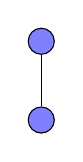
\begin{tikzpicture}[main/.style = {draw, circle, fill=blue!50}]
        \node[main] (0) {};
        \node[main] (1) [above of=0] {};
        %
        \draw (0) -- (1);
  \end{tikzpicture}}}
  \\

  \makecell{3} &
  \makecell{\boxed{
      
\begin{tikzpicture}[main/.style = {draw, circle, fill=blue!50}]
        \node[main] (0) {};
        \node[main] (1) [right of=0] {};
        \node[main] (2) [right of=1] {};
  \end{tikzpicture}}}

  \makecell{\boxed{
      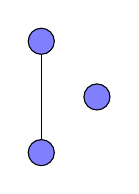
\begin{tikzpicture}[main/.style = {draw, circle, fill=blue!50}]
        \node[main] (0) {};
        \node[main] (1) [above right of=0] {};
        \node[main] (2) [above left of=1] {};
        %
        \draw (0) -- (2);
  \end{tikzpicture}}}

  \makecell{\boxed{
      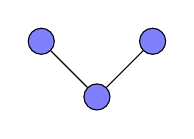
\begin{tikzpicture}[main/.style = {draw, circle, fill=blue!50}]
        \node[main] (0) {};
        \node[main] (1) [above right of=0] {};
        \node[main] (2) [above left of=0] {};
        %
        \draw (0) -- (2);
        \draw (0) -- (1);
  \end{tikzpicture}}}

  \makecell{\boxed{
      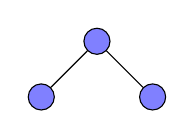
\begin{tikzpicture}[main/.style = {draw, circle, fill=blue!50}]
        \node[main] (0) {};
        \node[main] (1) [below right of=0] {};
        \node[main] (2) [below left of=0] {};
        %
        \draw (0) -- (2);
        \draw (0) -- (1);
  \end{tikzpicture}}}

  \makecell{\boxed{
      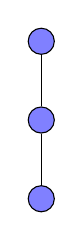
\begin{tikzpicture}[main/.style = {draw, circle, fill=blue!50}]
        \node[main] (0) {};
        \node[main] (1) [above of=0] {};
        \node[main] (2) [above of=1] {};
        %
        \draw (0) -- (1);
        \draw (1) -- (2);
  \end{tikzpicture}}}
  \\
  \makecell{\vdots} & \makecell{\vdots}\\
  \hline
\end{tabular}

\subsection{Maximal, Minimal, Greatest and Least elements}
For a Poset $(P, \le)$ we define the following:\\
$x \in P$ is maximal $\iff \forall y \in P, x \le y.~y \le x.$\\
$x \in P$ is minimal $\iff \forall y \in P, y \le x.~x \le y.$\\
$x \in P$ is greatest $\iff \forall y \in P.~y \le x.$\\
$x \in P$ is least $\iff \forall y \in P.~x \le y.$

Trivially, we can say that, $\forall (P, \le),~P \neq \emptyset,~n(P)
< \infty.~\exists \text{maximal}(P), \text{minimal}(P).$
Similarly, we can say that, there maybe at most a single greatest and
least elements of a poset. Not necessary for there to be one, but if
there is, then there can only be one.

\subsection{Induced Subposets}
Let $(P, \le)$ and $(Q, \le)$ be Posets s.t.\\
$Q \subset P$ and $\forall q_1, q_2 \in Q.~q_1 \le_Q q_2 \iff q_1
\le_P q_2$ then $Q$ is called an induced subposet of $P$.

Induced subposets are really useful for studying various isomorphism
classes and their relations (how one could go to another)

For example, consider the poset $(\bP, |)$ which is poset of Positive
integers, ordered by divisibility.
Subposets of $(\bP, |)$ of the form \\
$p, q\in \bP, \gcd(p, q) = 1, p \neq q. \left(\{p^a\cdot q^b \colon
a, b \in \bN \}, |\right)$\\
are isomorphic to the poset $(\bN^2, \le)$ where $(a, b) \le_{\bN^2}
(c, d) \iff a \leq_\bN c, b \leq_\bN d$.


More generally, if we fix $n$ distinct, pairwise coprime numbers: $(c_i)_{i=1}^n$.\\ 
Then, let\\
$(C_n, |)$ be $\left\{\prod c_i^{k_i} \colon \forall i.~k_i \in \bN.\right\}$ and,\\
$(\bN^n, \le)$ be a poset where $\le$ is defined by $(a_i)_{i=1}^n
\le (b_i)_{i=1}^n \iff \forall i \in [n].~a_i \le b_i$.

Then $(C_n, |) \cong (\bN^n, \le)$

\subsection{Incidence Algbera}
Let $(P, \le)$ be a Poset such that $\forall x, z \in P, n\left({y \in P \colon x \leq y \leq z}\right) < \infty$

Then we define\\
$A(P) := \{f\colon P \times P \to R \left| f(x, y) \neq 0 \implies x \leq y\right.\}$ and,\\
$*: A(P) \times A(P) \to A(P)$ as,
$$(f*g)(x, y) := \sum_{x \leq z \leq y} f(x, z) \cdot g(z, y)$$

\begin{theorem} $*$ is associative\end{theorem}

\begin{proof}
To prove that $\forall (P, \leq). \forall f,g,h \in A(P). (f * g) * h = f * (g * h)$.\\
Let's start by expanding the LHS and RHS.\\
LHS:
$$((f * g) * h)(x, z) = \sum_{x \leq y \leq z} (f * g)(x, y) \cdot h(y, z) = \sum_{x \leq y \leq z}\sum_{x \leq w \leq y}f(x,w)\cdot g(w,y) \cdot h(y,z)$$
RHS:
$$(f * (g * h))(x, z) = \sum_{x \leq y \leq z} f(x, y) \cdot (g * h)(y, z) = \sum_{x \leq y \leq z}\sum_{y \leq w \leq z}f(x,y)\cdot g(y,w) \cdot h(w,z)$$

Notice that\\
\begin{enumerate}
\item { On the LHS, we're traversing all the quadruplets $(x, y, w, z)$ such that $x \leq w \leq y \leq z$}
\item { On the RHS, we're traversing all the quadruplets $(x, w, y, z)$ such that $x \leq y \leq w \leq z$}
\end{enumerate}

Which simply means that, if we swap $w$ and $y$ on RHS it will be equivalent to the LHS.\\
\end{proof}

\end{document}
